\section*{Risk Treatment}
\addcontentsline{toc}{section}{Risk Treatment}

This part of the assessment aims at proposing a set of pre and post-incident security controls that can be found in figure \ref{fig:riskTreatCut2}. These controls are needed to lower the impact and the likelihood of an incident.

Regarding the main threats listed in the above section, the following main security controls were proposed

\begin{itemize}
    \item for \texttt{unauthorized wired connections} an intrusion prevention system to reduce the likelihood, and IP blacklist as post-control to reduce impact and avoid APT.
    \item for \texttt{hyperjacking} it is advisable to deploy the latest version of the hypervisor, implement a logical separation between guest and host machines, backup the configuration, and manage the hypervisor on a different port than the one used for hypervisor-guest communication\cite{online:virtualSec}. As post-controls, we can try and reset the admin credential, and restore the virtualization server with its backup, but if the access control is broken, then disaster recovery is needed.
    \item for \texttt{theft of equipment} the pre-controls consist of installing CCTV cameras, biometrical access control, and log personnel access. Since it's not reasonable to ask a municipality to install biometrical access control on a room that is used only when we are near the elections, we substituted this with a security officer.\cite{online:roomSec}
    \item for \texttt{router crashes} the main mitigations consist of implementing VRRP (Virtual Router Redundancy Protocol) \cite{online:VRRP} and configuration backup and restore when needed.
    \item finally, for \texttt{phishing campaigns} we need to train the personnel and implement anti-spam software on mail agents and SMTP servers to reduce the likelihood.
\end{itemize}

\begin{figure}[b!]
    \centering
    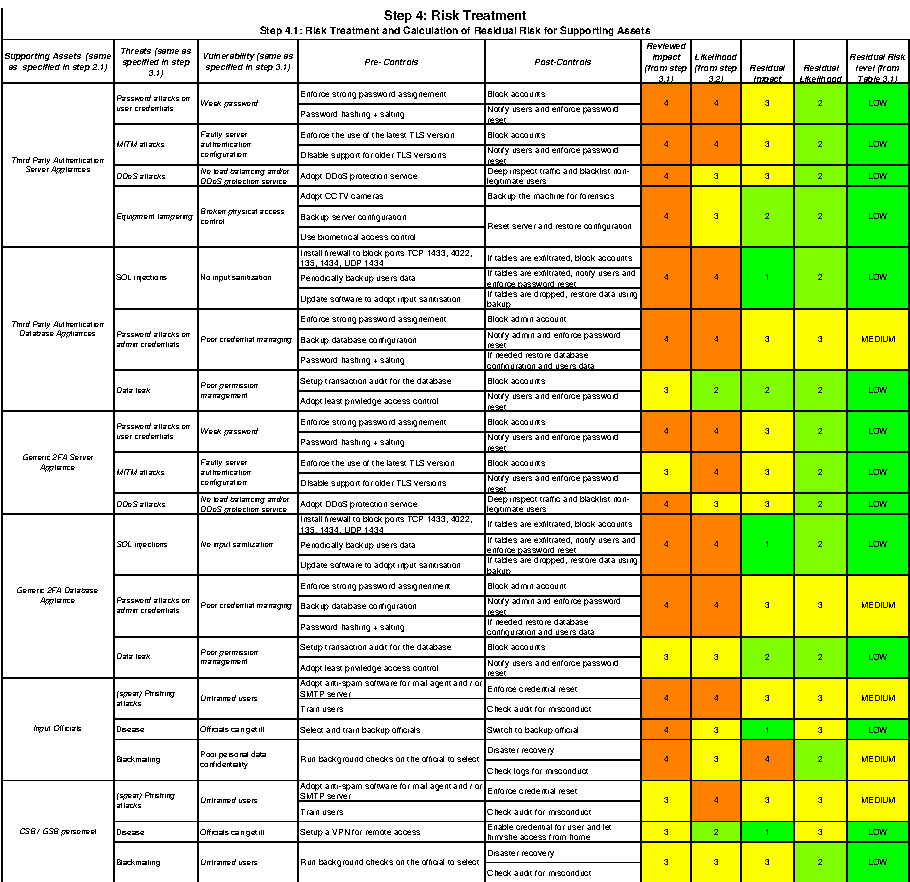
\includegraphics[keepaspectratio,width=1\textwidth]{03-risk-analysis/005-RT/img/riskTreatCut1.pdf}
    \label{fig:riskTreatCut1}
\end{figure}

\begin{figure}[t!]
    \centering
    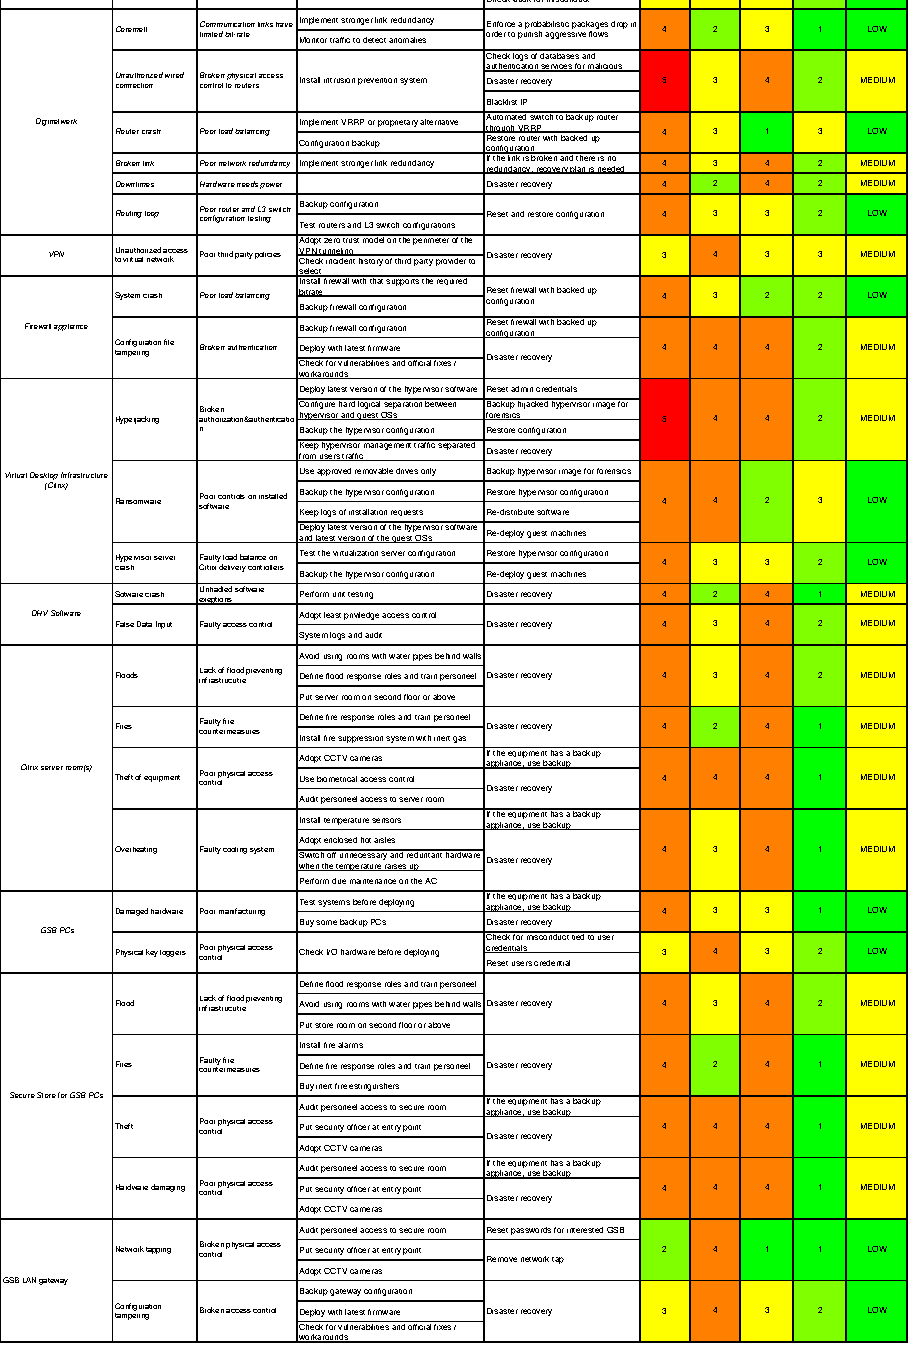
\includegraphics[keepaspectratio,width=1\textwidth]{03-risk-analysis/005-RT/img/riskTreatCut2.pdf}
    \caption{Risk treatment}
    \label{fig:riskTreatCut2}
\end{figure}

At the end of this step, no threats with high risk rating remained.

\noindent \textcolor{blue}{Update:}

\subsection*{Session Hijacking - CVE-2021-22927}

Citrix systems Inc. has already released an official patch with a reference guide on how to configure SAML. For this reason the vulnerability can be removed by upgrading the Citrix ADC software to version \texttt{13.0-82.41} or later, and by following the official configuration guide. \footnote{\href{https://support.citrix.com/article/CTX316577/citrix-application-delivery-controller-and-citrix-gateway-saml-configuration-reference-guide} {https://support.citrix.com/article/CTX316577/citrix-application-delivery-controller-and-citrix-gateway-saml-\\configuration-reference-guide}}

As a result, the impact is nulled.

\subsection*{Session Hijacking - CVE-2021-22927}


